%% Astronomy and Computing (Elsevier) Software / Infrastructure Paper
%% Built with Elsevier's official elsarticle class (author-year Harvard citations).
%% For final camera-ready layout, switch `preprint,12pt` to `final,5p,times,twocolumn,authoryear`.
\documentclass[preprint,12pt,authoryear]{elsarticle}

\usepackage{amsmath,amssymb}
\usepackage{booktabs}
\usepackage{graphicx}
\usepackage{hyperref}
\usepackage{lineno}
\usepackage{listings}
\usepackage{xcolor}
\usepackage{array}

\lstset{
  basicstyle=\ttfamily\small,
  breaklines=true,
  frame=single,
  backgroundcolor=\color{gray!8},
  rulecolor=\color{gray!40}
}

\journal{Astronomy and Computing}

\begin{document}

\begin{frontmatter}

\title{\texttt{specsynth}: Cloud-Native Distributed Infrastructure for Survey-Scale Astrophysical Spectral Synthesis}

\author[1]{Sankar Ganesh\corref{cor1}}
\ead{sankarganesh.astro@example.org} % TODO: replace with your preferred contact email before submission
\cortext[cor1]{Corresponding author. ORCID: 0009-0006-1590-1356.}

\affiliation[1]{organization={Independent Researcher},
                country={India}}

\begin{abstract}
Forward-modeling synthetic spectra and broadband photometry for $10^6$--$10^9$ simulated galaxies is a central computational bottleneck for wide-field cosmological surveys including Rubin LSST, \textit{Euclid}, and Roman. We present \texttt{specsynth}, an open-source Python framework that reformulates composite stellar population synthesis (SPS) as a cloud-native, out-of-core matrix-streaming pipeline built on chunked Zarr storage over \texttt{fsspec}, Dask task graphs, NumPy/OpenBLAS, and optional CuPy GPU contractions. Decoupling offline Simple Stellar Population (SSP) basis compilation from online chunked synthesis allows galaxy star formation histories to stream from local disks or cloud object stores (\texttt{s3://}, \texttt{gs://}, \texttt{abfs://}), undergo Charlot \& Fall two-component dust, Planck~2018 luminosity-distance scaling, and Madau IGM attenuation, and project in-flight into calibrated JWST, HST, and SDSS bandpasses without persisting multi-terabyte intermediate spectra. Against independent \texttt{float64} baselines, \texttt{float32} streaming achieves $9.87\times 10^{-7}$ maximum relative spectral error and $<3.0\times 10^{-7}$~mag photometric agreement across 16 filters. Empirically, \texttt{specsynth} sustains $57{,}978$~gal~s$^{-1}$ on a 12-core CPU, $258{,}812$~gal~s$^{-1}$ ($4.51\times$) on an NVIDIA Tesla T4 GPU, flat peak worker RAM (261.5--261.8~MB across $10^5$--$10^6$ galaxies), and $53{,}814$~gal~s$^{-1}$ on a 3-node Kubernetes cluster, alongside a four-tier quality sentry and a public 100,000-galaxy reference catalog (\texttt{DOI: 10.57967/hf/11635}).
\end{abstract}

%% Graphical abstract (optional for Astronomy and Computing; uncomment if desired)
%\begin{graphicalabstract}
%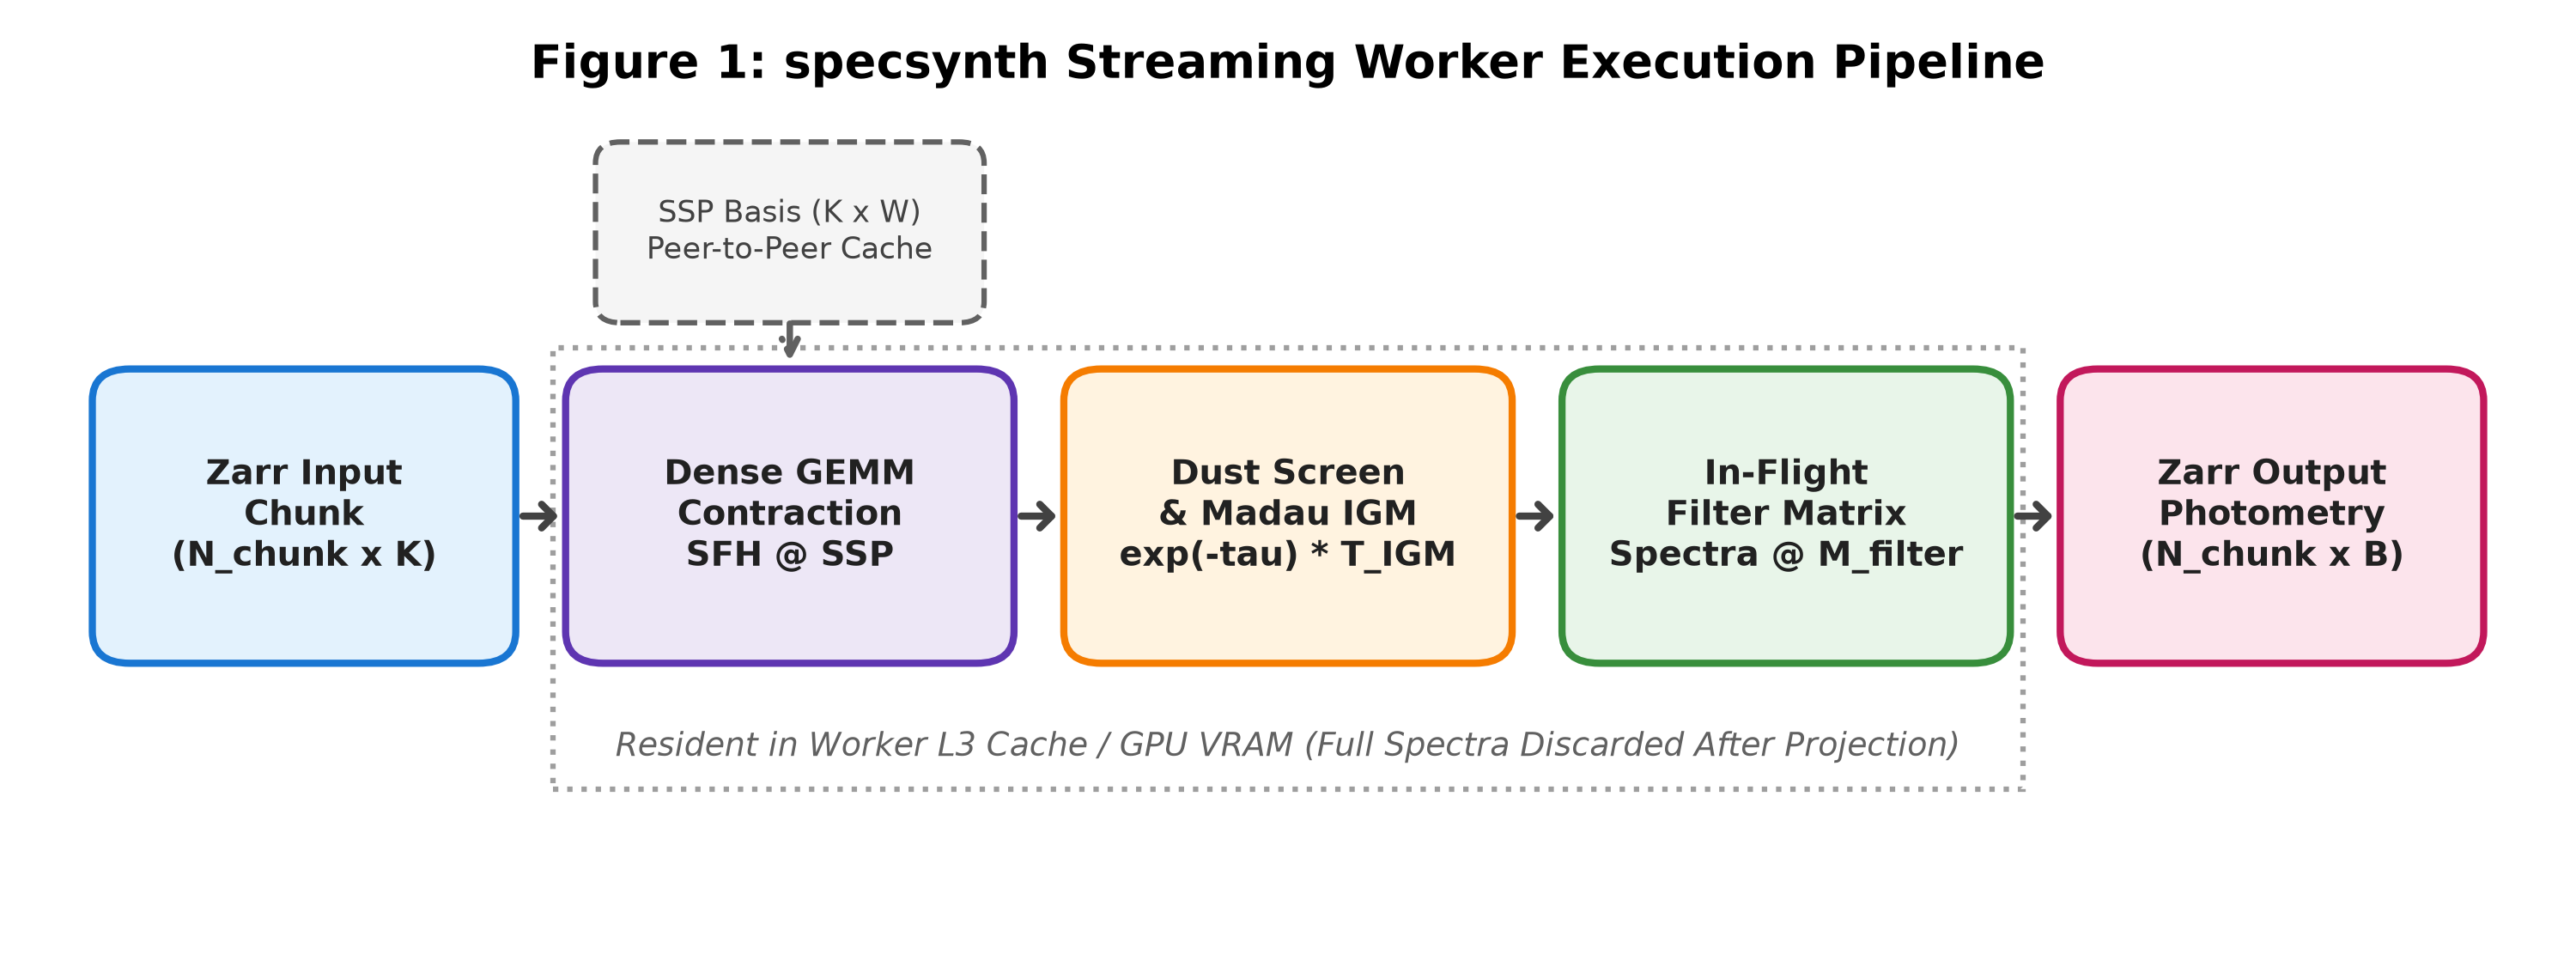
\includegraphics[width=\textwidth]{figures/fig1_pipeline.png}
%\end{graphicalabstract}

%% Research highlights: Elsevier requires 3-5 bullet points, strictly <= 85 chars each
\begin{highlights}
\item Cloud-native Dask/Zarr/CuPy engine projects photometry in-flight ($>99.9\%$ less I/O)
\item Peak worker RAM stays flat at 261.5--261.8~MB streaming $10^5$--$10^6$ galaxies
\item Reaches 258.8k~gal/s on Tesla T4 GPU ($4.51\times$) and 53.8k~gal/s on 3-node K8s
\item Matches float64 to $9.87\times 10^{-7}$ spectral and $<3\times 10^{-7}$~mag error
\end{highlights}

\begin{keyword}
Stellar population synthesis \sep Synthetic photometry \sep Distributed computing \sep Cloud object storage \sep Dask \sep Zarr
\end{keyword}

\end{frontmatter}

\linenumbers

%% =========================================================================
\section{Introduction and Statement of Need}
\label{sec:intro}

Interpreting next-generation wide-field extragalactic surveys---including the Vera C. Rubin Observatory Legacy Survey of Space and Time \citep[LSST;][]{ivezic2019lsst}, the \textit{Euclid} mission \citep{mellier2025euclid}, and the Nancy Grace Roman Space Telescope \citep{akeson2019wfirst}---requires translating cosmological hydrodynamical simulations such as IllustrisTNG \citep{pillepich2018simulating} and large semi-analytic mock catalogs ($10^6$--$10^9$ simulated galaxies) into survey-ready synthetic spectra and broadband photometry. Performing this forward-modeling transformation at survey scale exposes three recurring systems bottlenecks:

\begin{enumerate}
\item \textbf{Intermediate Storage Explosion:} Evaluating high-resolution composite spectra ($W \approx 2{,}000$--$10{,}000$ wavelength bins) for $10^8$ galaxies produces multiple terabytes of intermediate spectral arrays that are routinely discarded immediately after integrating into 5--16 photometric bandpasses.
\item \textbf{Memory and Serialization Overhead:} Wrapping stateful single-galaxy Fortran/C integrators inside parallel loops duplicates per-worker model state and forces shared POSIX filesystems (NFS/Lustre), whereas monolithic in-memory NumPy arrays \citep{harris2020array} rapidly exhaust host RAM or GPU VRAM as catalog sizes grow.
\item \textbf{Silent Catalog Corruption at Scale:} Manual inspection of individual spectral energy distributions (SEDs) is infeasible across millions of simulated subhalos, allowing unphysical edge cases (negative masses, zero-metallicity singularities, negative fluxes, or out-of-range spectral breaks) to propagate silently into downstream cosmological analyses.
\end{enumerate}

\texttt{specsynth} is an open-source Python framework built to solve these systems challenges. Rather than introducing a new stellar evolution model, \texttt{specsynth} reformulates composite stellar population synthesis as a cloud-native, linear matrix-streaming pipeline built on chunked Zarr storage over \texttt{fsspec}, Dask distributed task graphs \citep{rocklin2015dask}, NumPy/OpenBLAS \citep{harris2020array}, and optional CuPy GPU contractions \citep{okuta2017cupy}. Galaxy star formation histories (SFHs) stream from local storage or cloud object stores (\texttt{s3://}, \texttt{gs://}, \texttt{abfs://}), contract against cached Simple Stellar Population (SSP) basis matrices in worker L3 cache or VRAM, undergo dust and intergalactic medium (IGM) attenuation, and project directly into photometric bandpasses in-flight without persisting multi-terabyte intermediate spectra.

%% =========================================================================
\section{State of the Field and Architectural Comparison}
\label{sec:sota}

The astrophysical SPS and distributed-computing ecosystem spans several mature software paradigms, each optimized for distinct scientific workflows:

\begin{itemize}
\item \textbf{Single-Galaxy Precision and Bayesian SED Inference:} Foundational codes such as FSPS \citep{conroy2009propagation} and BC03 \citep{bruzual2003stellar} provide stellar evolution libraries and high-precision spectral integrators, while \texttt{Prospector} \citep{johnson2021prospector} and \texttt{BAGPIPES} \citep{carnall2018bagpipes} wrap them for Bayesian parameter inference on observed galaxies. Wrapping per-galaxy Fortran/C integrators inside parallel loops (e.g., via \texttt{mpi4py} or \texttt{dask.bag.map}) duplicates stateful model memory across cores, incurs initialization overhead, and assumes shared POSIX filesystems.
\item \textbf{Differentiable and Neural Emulator Frameworks:} \texttt{DSPS} \citep{hearin2023dsps} provides JAX-based differentiable SPS for gradient-driven inference and fast GPU evaluation, while \texttt{SPECULATOR} \citep{alsing2020speculator} trains neural surrogates for millisecond spectral approximation. However, \texttt{DSPS} targets in-memory JAX device buffers rather than distributed cloud object-store streaming, and neural emulators introduce surrogate approximation errors and require retraining whenever SSP grids, IMFs, or dust laws change.
\item \textbf{Object-Oriented Synthetic Observable Frameworks:} \texttt{Synthesizer} \citep{lovell2025synthesizer,roper2026synthesizer} provides a comprehensive Python framework for generating synthetic spectra, nebular emission lines, images, and photometry from cosmological simulations using rich galaxy, grid, and photoionization abstractions.
\item \textbf{General-Purpose Distributed Data Engines:} Engines such as Apache Spark \citep{zaharia2016apache} and Ray \citep{moritz2018ray} excel at relational joins, row-level ETL, and distributed ML, but incur JVM--Python serialization overhead or require custom pipeline engineering to combine zero-copy BLAS/CuPy contractions with chunked Zarr streaming.
\end{itemize}

\begin{table*}[t]
\centering
\caption{Architectural comparison between \texttt{specsynth} and alternative paradigms for survey-scale galaxy spectral and photometric forward-modeling.}
\label{tab:arch_comparison}
\footnotesize
\setlength{\tabcolsep}{4pt}
\begin{tabular}{@{}p{2.5cm}p{2.9cm}p{2.9cm}p{2.9cm}p{3.4cm}@{}}
\toprule
\textbf{Dimension} & \textbf{SPS Wrappers (FSPS + MPI)} & \textbf{Differentiable / Emulators (DSPS / SPECULATOR)} & \textbf{Big Data Engines (Spark / Ray)} & \textbf{\texttt{specsynth} (This Work)} \\
\midrule
Physics vs.\ Execution & Coupled per-galaxy integration & Auto-diff or neural surrogate & Physics-agnostic & Decoupled offline $K\times W$ basis, online streaming GEMM \\
Storage Backend & POSIX filesystem (NFS / Lustre) & Host RAM / GPU VRAM buffers & HDFS / Object store (JVM) & Native cloud object store (\texttt{s3://}, \texttt{gs://}, \texttt{abfs://}) via Zarr/\texttt{fsspec} \\
Worker Memory & Large stateful model per core & Bounded by GPU VRAM (OOM risk) & Serialization and shuffle overhead & Strictly bounded to one chunk, $O(N_{\text{chunk}} \times W)$ \\
In-Flight Filter Projection & No (retains or writes spectra) & Custom tensor ops & Requires custom pipeline stages & Native in-cache / VRAM projection; $>99.9\%$ storage reduction \\
GPU Acceleration & CPU only & Yes (JAX / PyTorch) & Requires specialized plugins & CuPy/cuBLAS with transparent OpenBLAS CPU fallback \\
\bottomrule
\end{tabular}
\end{table*}

\textbf{Build vs.\ Contribute Rationale:} Rather than re-implementing nebular photoionization or Bayesian SED fitting already well served by \texttt{Synthesizer}, \texttt{Prospector}, and \texttt{DSPS}, \texttt{specsynth} is designed as a focused, lightweight execution engine targeting a narrower systems problem: strictly memory-bounded, out-of-core Zarr/Dask/CuPy streaming with in-flight filter contraction, zero shared-filesystem requirements, and integrated catalog-scale quality auditing. Because \texttt{specsynth} ingests standardized $(K, W)$ SSP matrices through pluggable adapters---including BC03 \citep{bruzual2003stellar}, E-MILES \citep{vazdekis2016uv}, FSPS \citep{conroy2009propagation}, BPASS \citep{eldridge2017binary}, and generic FITS/HDF5/NPZ grids---it complements upstream SPS libraries and simulation frameworks (Table~\ref{tab:arch_comparison}).

%% =========================================================================
\section{Astrophysical Forward-Modeling Framework}
\label{sec:physics}

Importantly, \texttt{specsynth} does not introduce new stellar evolutionary tracks; it provides a verified, cloud-native execution architecture for scaling existing SSP models to survey volumes.

\subsection{Two-Component Composite Stellar Synthesis}
For each galaxy $g$, composite rest-frame flux density follows the \citet{charlot2000simple} two-component dust attenuation law:
\begin{equation}
\label{eq:cf00}
F_g(\lambda) = D_g(\lambda)\!\left[\sum_{k \in \text{old}} \mathrm{SFH}[g,k]\,\mathrm{SSP}[k,\lambda] + B_g(\lambda)\sum_{k \in \text{young}} \mathrm{SFH}[g,k]\,\mathrm{SSP}[k,\lambda]\right],
\end{equation}
where $\mathrm{SFH}[g,k]$ is the stellar mass formed in age--metallicity grid cell $k$ and $\mathrm{SSP}[k,\lambda]$ is the intrinsic stellar luminosity per unit mass. Stellar populations younger than $10^7$~yr experience additional birth-cloud attenuation $B_g(\lambda)$ atop diffuse interstellar medium (ISM) attenuation $D_g(\lambda)$:
\begin{align}
D_g(\lambda) &= \exp\!\left[-\tau_{\text{diffuse}}\left(\frac{\lambda}{5500\,\text{\AA}}\right)^{\alpha_{\text{diffuse}}}\right], \label{eq:diffuse} \\
B_g(\lambda) &= \exp\!\left[-\tau_{\text{birth}}\left(\frac{\lambda}{5500\,\text{\AA}}\right)^{\alpha_{\text{birth}}}\right]. \label{eq:birth}
\end{align}
Separating the age--metallicity basis into young ($k \in \text{young}$) and old ($k \in \text{old}$) contiguous index partitions transforms Eq.~\eqref{eq:cf00} over a chunk of $N_{\text{chunk}}$ galaxies into two dense matrix multiplications (GEMM) followed by vectorized elementwise attenuation screens.

\subsection{Cosmology, IGM Absorption, and Calibrated Photometry}
\texttt{specsynth} supports both uniform cosmological snapshots (single redshift $z$) and lightcone forward-modeling (per-galaxy redshifts $z_g$). Rest-frame wavelengths shift via $\lambda_{\text{obs}} = \lambda_{\text{rest}}(1+z)$ with luminosity-distance dimming evaluated using \texttt{specsynth.cosmology.FlatLambdaCDM} (Planck~2018 defaults: $H_0 = 67.4\;\mathrm{km\,s^{-1}\,Mpc^{-1}}$, $\Omega_{m,0} = 0.315$):
\begin{equation}
F_{\lambda,\text{obs}}(\lambda_{\text{obs}}) = \frac{L_{\lambda}(\lambda_{\text{obs}} / (1+z))}{4\pi D_L(z)^2 (1+z)}\,T_{\text{IGM}}(\lambda_{\text{obs}}, z).
\end{equation}
Intergalactic neutral hydrogen absorption uses the \citet{madau1995radiative} transmission model,
\begin{equation}
T_{\text{IGM}}(\lambda_{\text{obs}}, z) = \exp\!\left[-\tau_{\text{lines}}(\lambda_{\text{obs}}, z) - \tau_{\text{continuum}}(\lambda_{\text{obs}}, z)\right],
\end{equation}
integrating resonant Lyman-series transitions shortward of Ly$\alpha$ ($1215.67\,\text{\AA}$) through the Lyman continuum limit ($911.75\,\text{\AA}$). Broadband photometry is computed via photon-weighted bandpass integration against bundled calibrated STScI/SDSS throughput curves---7 JWST NIRCam bands (\texttt{F090W}--\texttt{F444W}), 4 HST ACS/WFC3 bands (\texttt{F435W}, \texttt{F606W}, \texttt{F814W}, \texttt{F160W}), and 5 SDSS bands ($u, g, r, i, z$)---as well as user-supplied empirical filter tables and analytical super-Gaussian approximations (\texttt{\_approx}) for rapid prototyping.

%% =========================================================================
\section{Software Architecture and Engineering Implementation}
\label{sec:architecture}

\texttt{specsynth} decouples offline SSP grid compilation from online chunked synthesis so that worker memory remains strictly $O(N_{\text{chunk}} \times W)$ independent of total catalog size (Figure~\ref{fig:pipeline}).

\begin{figure}[t]
\centering
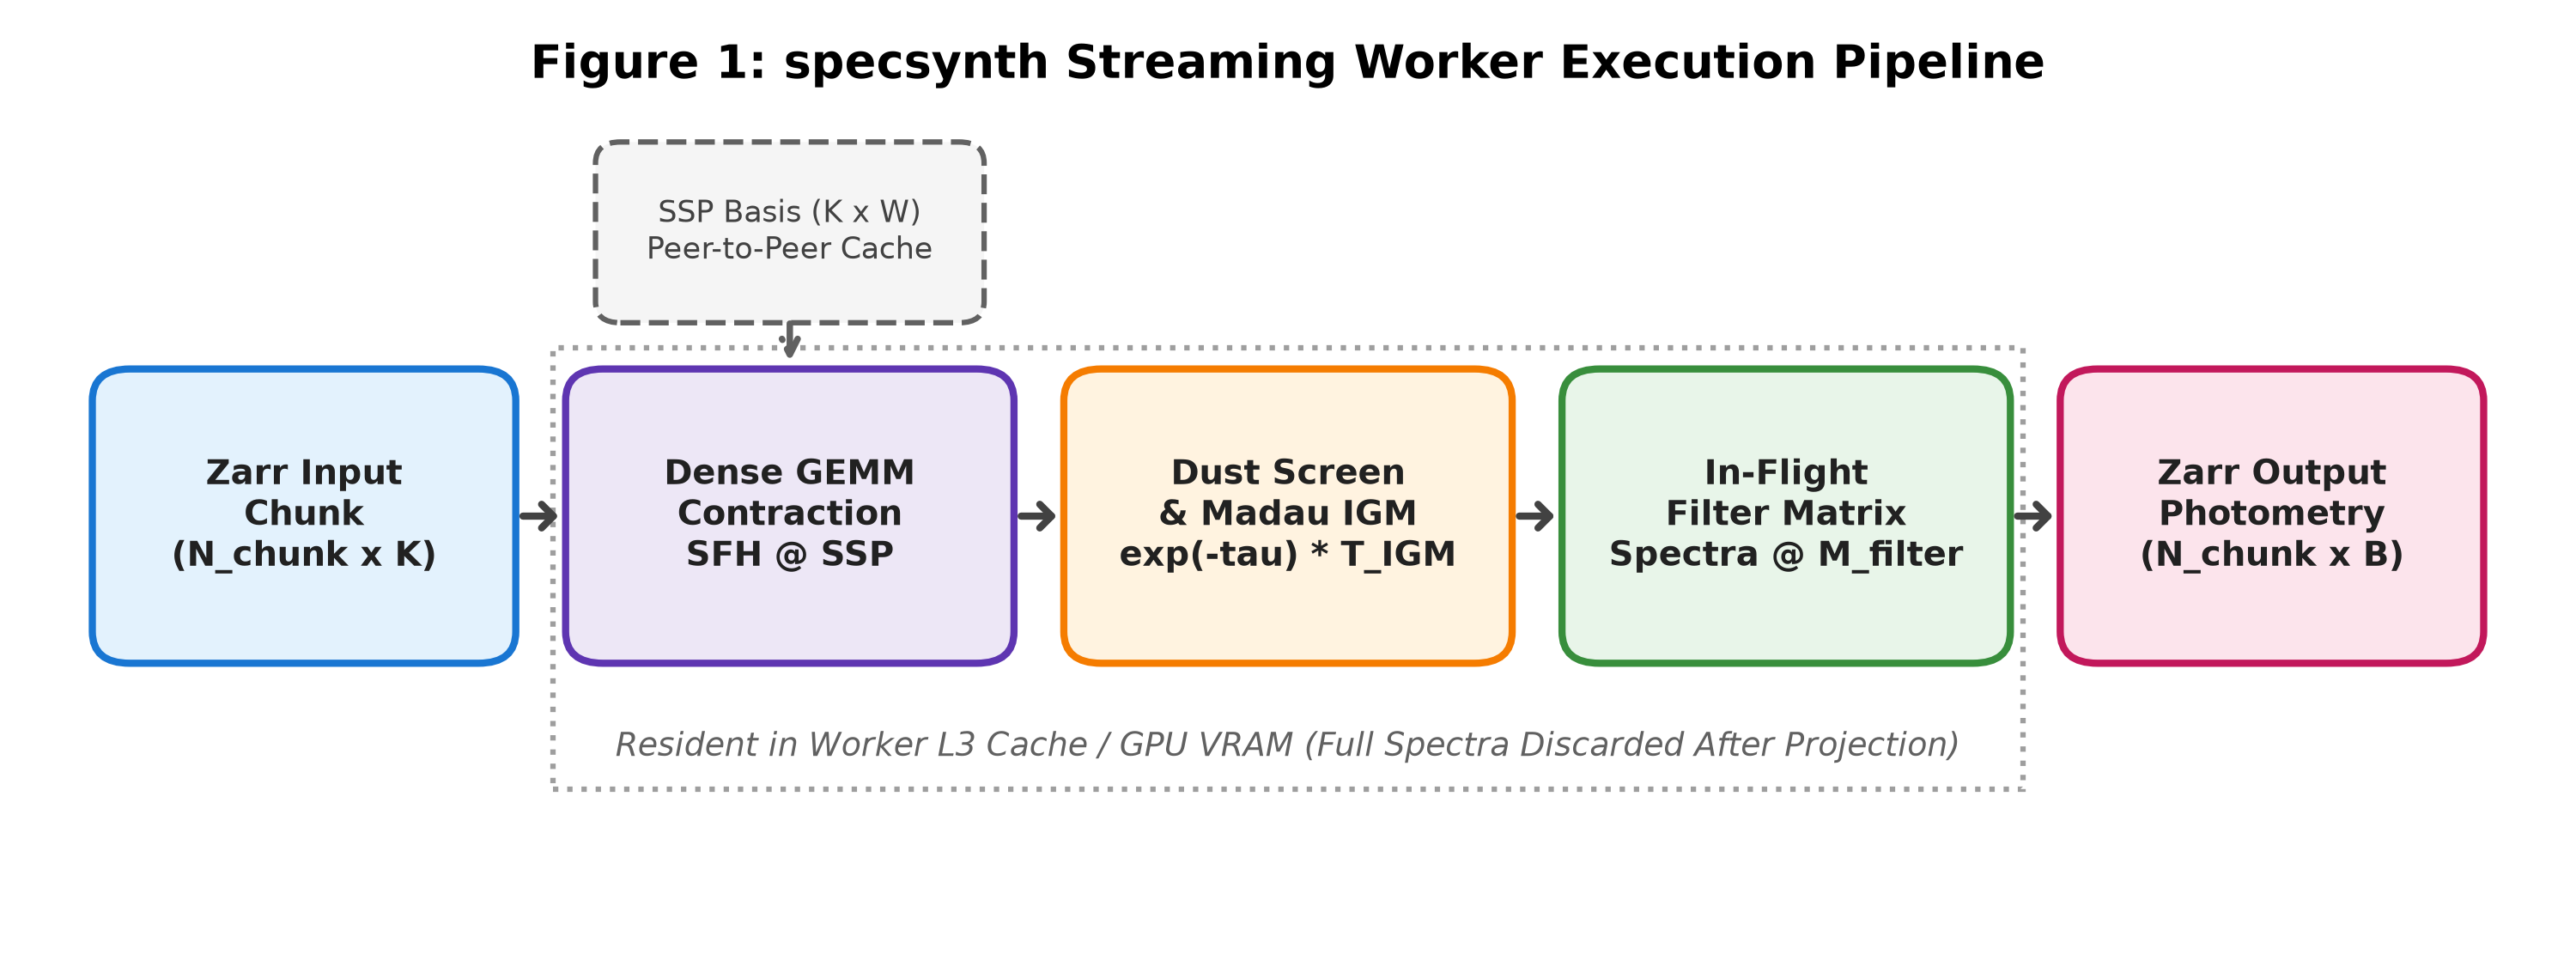
\includegraphics[width=\textwidth]{figures/fig1_pipeline.png}
\caption{Streaming worker execution pipeline of \texttt{specsynth}. The immutable $(K\times W)$ SSP basis is cached once per worker, while galaxy chunks $(N_{\text{chunk}} \times K)$ stream from local or cloud Zarr storage through dense \texttt{float32} GEMM contractions, Charlot \& Fall dust and Madau IGM attenuation, and in-flight filter projection before full spectra are discarded.}
\label{fig:pipeline}
\end{figure}

\subsection{Core Subsystem Design}
\begin{enumerate}
\item \textbf{Pluggable SSP Library Adapters (\texttt{specsynth.adapters}):} Standardized adapters compile raw spectral libraries into immutable Zarr basis matrices $(K \times W)$ with 100\% automated unit-test coverage:
  \begin{itemize}
  \item \emph{Bruzual \& Charlot (2003):} Parses Fortran unformatted sequential binary records (\texttt{.ised}) and multi-metallicity ASCII tables \citep{bruzual2003stellar}.
  \item \emph{E-MILES / MILES:} Ingests single- and multi-file FITS libraries \citep{vazdekis2016uv} with automatic wavelength interpolation and a built-in pure-Python fallback FITS reader for minimal container environments lacking \texttt{astropy}.
  \item \emph{FSPS and BPASS:} Supports programmatic generation via \texttt{python-fsps} \citep{conroy2009propagation}, direct parsing of raw Fortran ASCII outputs (\texttt{spstot\_*.spec}), and tabular ingestion for BPASS \citep{eldridge2017binary}.
  \item \emph{Generic FITS/HDF5/NPZ Grids:} Multi-dimensional adapter with automatic age-unit inference (linear years, $\log_{10}(\mathrm{yr})$, or Gyr) across primary image arrays and binary table columns.
  \end{itemize}
\item \textbf{In-Flight Filter Projection:} When broadband photometry is requested (\texttt{--filters} or \texttt{--bands}), chunk spectra $\mathbf{F}_{\text{chunk}} \in \mathbb{R}^{N_{\text{chunk}} \times W}$ are contracted in-flight against a \texttt{float64}-normalized projection matrix $\mathbf{M}_{\text{filter}} \in \mathbb{R}^{W \times B}$:
  \begin{equation}
  \mathbf{Phot}_{\text{chunk}} = \mathbf{F}_{\text{chunk}}\,\mathbf{M}_{\text{filter}}.
  \end{equation}
  Full chunk spectra remain resident in CPU L3 cache or GPU VRAM and are immediately discarded, reducing persistent storage by $>99.9\%$ (e.g., $3.2$~GB vs.\ $3.2$~TB for $10^8$ galaxies across 8 bands at $W=2{,}000$).
\item \textbf{Mixed-Precision Engineering Trade-off:} Matrix contractions run in \texttt{float32} to halve memory bandwidth and double SIMD/VRAM throughput, while cosmological distance integration and bandpass normalization remain in \texttt{float64}.
\item \textbf{Multi-Format Catalog Ingestion (\texttt{import-catalog}):} Streams cosmological simulation catalogs from Parquet, FITS, HDF5, CSV, and NPZ formats (compatible with IllustrisTNG, EAGLE, CAMELS, and SAM schemas) directly into chunked Zarr arrays.
\item \textbf{Scheduler Boundedness and Adaptive Chunking:} For survey catalogs with $N \ge 10^8$ galaxies, naive Dask task graphs bloat centralized scheduler RAM. \texttt{specsynth} provides adaptive chunk sizing (\texttt{compute\_adaptive\_chunk\_size}), dynamic CPU core budgeting, an automatic graph guard ($<25{,}000$ tasks), and sliding-window batched Zarr writes (\texttt{--batch-chunks}) that bound scheduler memory strictly to $O(B)$ active chunks.
\end{enumerate}

\subsection{Four-Tier Scientific Sentry and Autonomous QA}
To guard against silent catalog corruption across millions of simulated subhalos without interrupting cluster runs, \texttt{specsynth} embeds a four-tier diagnostic quality sentry (\texttt{specsynth.sentry}) and remediation agent (\texttt{specsynth.agent}):
\begin{itemize}
\item \textbf{Tier 1 (Fast Numerical Invariants):} Vectorized masks trap non-finite values (\texttt{NaN}/$\pm\infty$), non-positive fluxes ($F \le 0$), and dust energy-conservation violations ($\int F_{\text{att}}\,d\lambda > (1+10^{-6})\int F_{\text{int}}\,d\lambda$).
\item \textbf{Tier 2 (Physical and Spectral Diagnostics):} Evaluates the narrowband $D_n(4000)$ break ($0.95 \le D_n4000 \le 2.50$), UV continuum slope $\beta_{\text{UV}}$ ($-2.80 \le \beta_{\text{UV}} \le +1.50$), and apparent AB magnitude bounds ($10.0 \le m_{\text{AB}} \le 35.0$).
\item \textbf{Tier 3 (Population Statistical Validation):} Monitors color--magnitude dispersion and bimodality to detect silent population collapse into degenerate constant vectors.
\item \textbf{Tier 4 (Quarantine, Remediation, and Out-of-Core Tooling):} Isolates flagged galaxy indices into \texttt{sentry\_quarantine/} alongside \texttt{is\_valid} Zarr masks without aborting distributed execution. \texttt{SentryAgent} (\texttt{specsynth sentry-agent}) clusters root causes (\texttt{STARBURST\_SLOPE\_EXTREME}, \texttt{DUST\_ZERO\_INFRARED\_EXCESS}, \texttt{INPUT\_MASS\_ZERO\_UNDERFLOW}) and produces certified catalogs (\texttt{specsynth clean-catalog}), while \texttt{specsynth.tools} exposes out-of-core slice inspection for external analysis and agent workflows.
\end{itemize}

%% =========================================================================
\section{Verification, Empirical Benchmarks, and Scaling Analysis}
\label{sec:benchmarks}

To prevent conflation between directly executed hardware benchmarks and multi-node extrapolations, we explicitly separate \emph{Empirical Measurements} (Sections~\ref{sec:correctness}--\ref{sec:multinode}) from \emph{Analytical Scaling and Cost Projections} (Section~\ref{sec:analytical}). All empirical figures are recorded in machine-readable JSON manifests under \texttt{paper/} in the repository.

\subsection{Numerical Correctness and Cross-Code Validation}
\label{sec:correctness}
We validated \texttt{specsynth} against independent serial \texttt{float64} baselines across three complementary checks (Table~\ref{tab:correctness}):
\begin{enumerate}
\item \emph{Full-Spectrum Contraction:} Over 2,000 galaxies ($K=60$, $W=1{,}200$; \texttt{paper/benchmark\_manifest.json}), \texttt{float32} streaming matches the serial \texttt{float64} reference to a maximum relative error of $9.87\times 10^{-7}$ (mean $8.77\times 10^{-8}$, median $7.21\times 10^{-8}$, RMSE $2.24\times 10^{-11}$).
\item \emph{16-Band Photometric Fidelity:} Using \texttt{scripts/cross\_validate\_sps.py} (\texttt{paper/cross\_validation\_manifest.json}) on a 500-galaxy IllustrisTNG-like population at $z=2.0$, maximum photometric residuals across all 16 calibrated bands stay below $3.0\times 10^{-7}$~mag---over three orders of magnitude tighter than the $10^{-3}$~mag survey target.
\item \emph{Cosmological Distances:} Across $z \in [0.05, 6.0]$, \texttt{FlatLambdaCDM} comoving and luminosity distances match independent 2,000-node FLRW quadrature to $8.51\times 10^{-14}$ (Planck~2018) and $8.23\times 10^{-14}$ (concordance $\Lambda$CDM). Optional live hooks for \texttt{python-fsps} and \texttt{DSPS} are included in the validation script when those packages are installed.
\end{enumerate}

\begin{table}[t]
\centering
\caption{Empirical numerical verification metrics for \texttt{specsynth} against independent \texttt{float64} reference implementations.}
\label{tab:correctness}
\small
\begin{tabular}{@{}llcc@{}}
\toprule
\textbf{Validation Check} & \textbf{Metric} & \textbf{Measured Value} & \textbf{Tolerance} \\
\midrule
Spectral Contraction ($N=2{,}000$, $W=1{,}200$) & Max rel.\ error & $9.87\times 10^{-7}$ & $< 5.0\times 10^{-4}$ \\
 & Mean / Median rel.\ error & $8.77\times 10^{-8}$ / $7.21\times 10^{-8}$ & $< 1.0\times 10^{-5}$ \\
 & RMSE & $2.24\times 10^{-11}$ & --- \\
\addlinespace
16-Band Photometry ($N=500$, $z=2.0$) & JWST NIRCam (7 bands) max $|\Delta m_{\mathrm{AB}}|$ & $1.57\times 10^{-7}$~mag & $< 10^{-3}$~mag \\
 & HST ACS/WFC3 (4 bands) max $|\Delta m_{\mathrm{AB}}|$ & $2.96\times 10^{-7}$~mag & $< 10^{-3}$~mag \\
 & SDSS $ugriz$ (5 bands) max $|\Delta m_{\mathrm{AB}}|$ & $2.61\times 10^{-7}$~mag & $< 10^{-3}$~mag \\
 & Median $|\Delta m_{\mathrm{AB}}|$ across sets & $0.98$--$1.39\times 10^{-8}$~mag & $< 10^{-3}$~mag \\
\addlinespace
Cosmology ($z \in [0.05, 6.0]$) & Planck~2018 $D_L(z)$ max rel.\ error & $8.51\times 10^{-14}$ & $< 10^{-4}$ \\
 & Concordance $\Lambda$CDM $D_L(z)$ max rel.\ error & $8.23\times 10^{-14}$ & $< 10^{-4}$ \\
\bottomrule
\end{tabular}
\end{table}

\subsection{Single-Node CPU BLAS vs.\ NVIDIA Tesla T4 GPU Throughput}
\label{sec:gpu}
Table~\ref{tab:throughput} compares single-node execution across five timed runs (after two warmups) on a standardized workload of $N=50{,}000$ galaxies, $K=60$ SSP templates, and $W=1{,}200$ wavelength bins ($14.76$~GFLOPs total). On an NVIDIA Tesla T4 GPU (14.56~GB VRAM, CUDA~12.2, CuPy~13.3.0), \texttt{specsynth} synthesizes 50,000 galaxies in $0.1932\pm 0.0040$~s---a $4.51\times$ measured speedup over the same cloud VM's CPU BLAS backend ($1.22$~GB~s$^{-1}$ vs.\ $0.27$~GB~s$^{-1}$ effective bandwidth). A public reproducible GPU notebook is archived on Kaggle.\footnote{\url{https://www.kaggle.com/code/bsankarganesh/specsynth-gpu-benchmark}}

\begin{table*}[t]
\centering
\caption{Measured single-node CPU BLAS vs.\ NVIDIA Tesla T4 GPU throughput ($N=50{,}000$, $K=60$, $W=1{,}200$, 5 timed runs after 2 warmups).}
\label{tab:throughput}
\small
\begin{tabular}{@{}llcccc@{}}
\toprule
\textbf{Hardware Environment} & \textbf{Backend} & \textbf{Mean Time (s)} & \textbf{Throughput (gal/s)} & \textbf{Rate (GFLOPS)} & \textbf{Speedup} \\
\midrule
Workstation CPU (Intel 12C/14T) & \texttt{scipy-openblas} & $0.8624 \pm 0.0577$ & 57,978 & 17.12 & $1.00\times$ (Local) \\
Cloud VM CPU (Linux 2C/4T) & \texttt{scipy-openblas} & $0.8719 \pm 0.0252$ & 57,344 & 16.93 & $1.00\times$ (Cloud) \\
Cloud GPU (NVIDIA Tesla T4) & CuPy 13.3 / CUDA 12.2 & $0.1932 \pm 0.0040$ & \textbf{258,812} & \textbf{76.40} & \textbf{4.51$\times$} \\
\bottomrule
\end{tabular}
\end{table*}

\subsection{Out-of-Core Memory Boundedness}
\label{sec:memory}
Kernel working-set tracking (\texttt{psutil}) while streaming $100{,}000$ to $1{,}000{,}000$ galaxies sequentially in 20,000-galaxy chunks confirms strict $O(N_{\text{chunk}} \times W)$ boundedness (Table~\ref{tab:memory}, Figure~\ref{fig:memory}). Across a $10\times$ catalog expansion, peak worker resident set size (RSS) varied by less than $0.2\%$ ($261.5$--$261.8$~MB) with zero disk spill, compared to $14.90$~GB required to hold unchunked $W=4{,}000$ \texttt{float32} spectra in RAM.

\begin{table}[t]
\centering
\caption{Measured peak worker resident RAM (RSS) during chunked streaming ($N_{\text{chunk}} = 20{,}000$) compared against monolithic in-memory spectral allocation ($W=4{,}000$, \texttt{float32}).}
\label{tab:memory}
\small
\begin{tabular}{@{}rcc@{}}
\toprule
\textbf{Streamed Catalog Size} & \textbf{Measured Peak Worker RSS} & \textbf{Monolithic Spectra Footprint} \\
\midrule
100,000 galaxies & 261.5~MB & 1.49~GB \\
250,000 galaxies & 261.5~MB & 3.73~GB \\
500,000 galaxies & 261.5~MB & 7.45~GB \\
1,000,000 galaxies & 261.8~MB & 14.90~GB \\
\bottomrule
\end{tabular}
\end{table}

\begin{figure}[t]
\centering
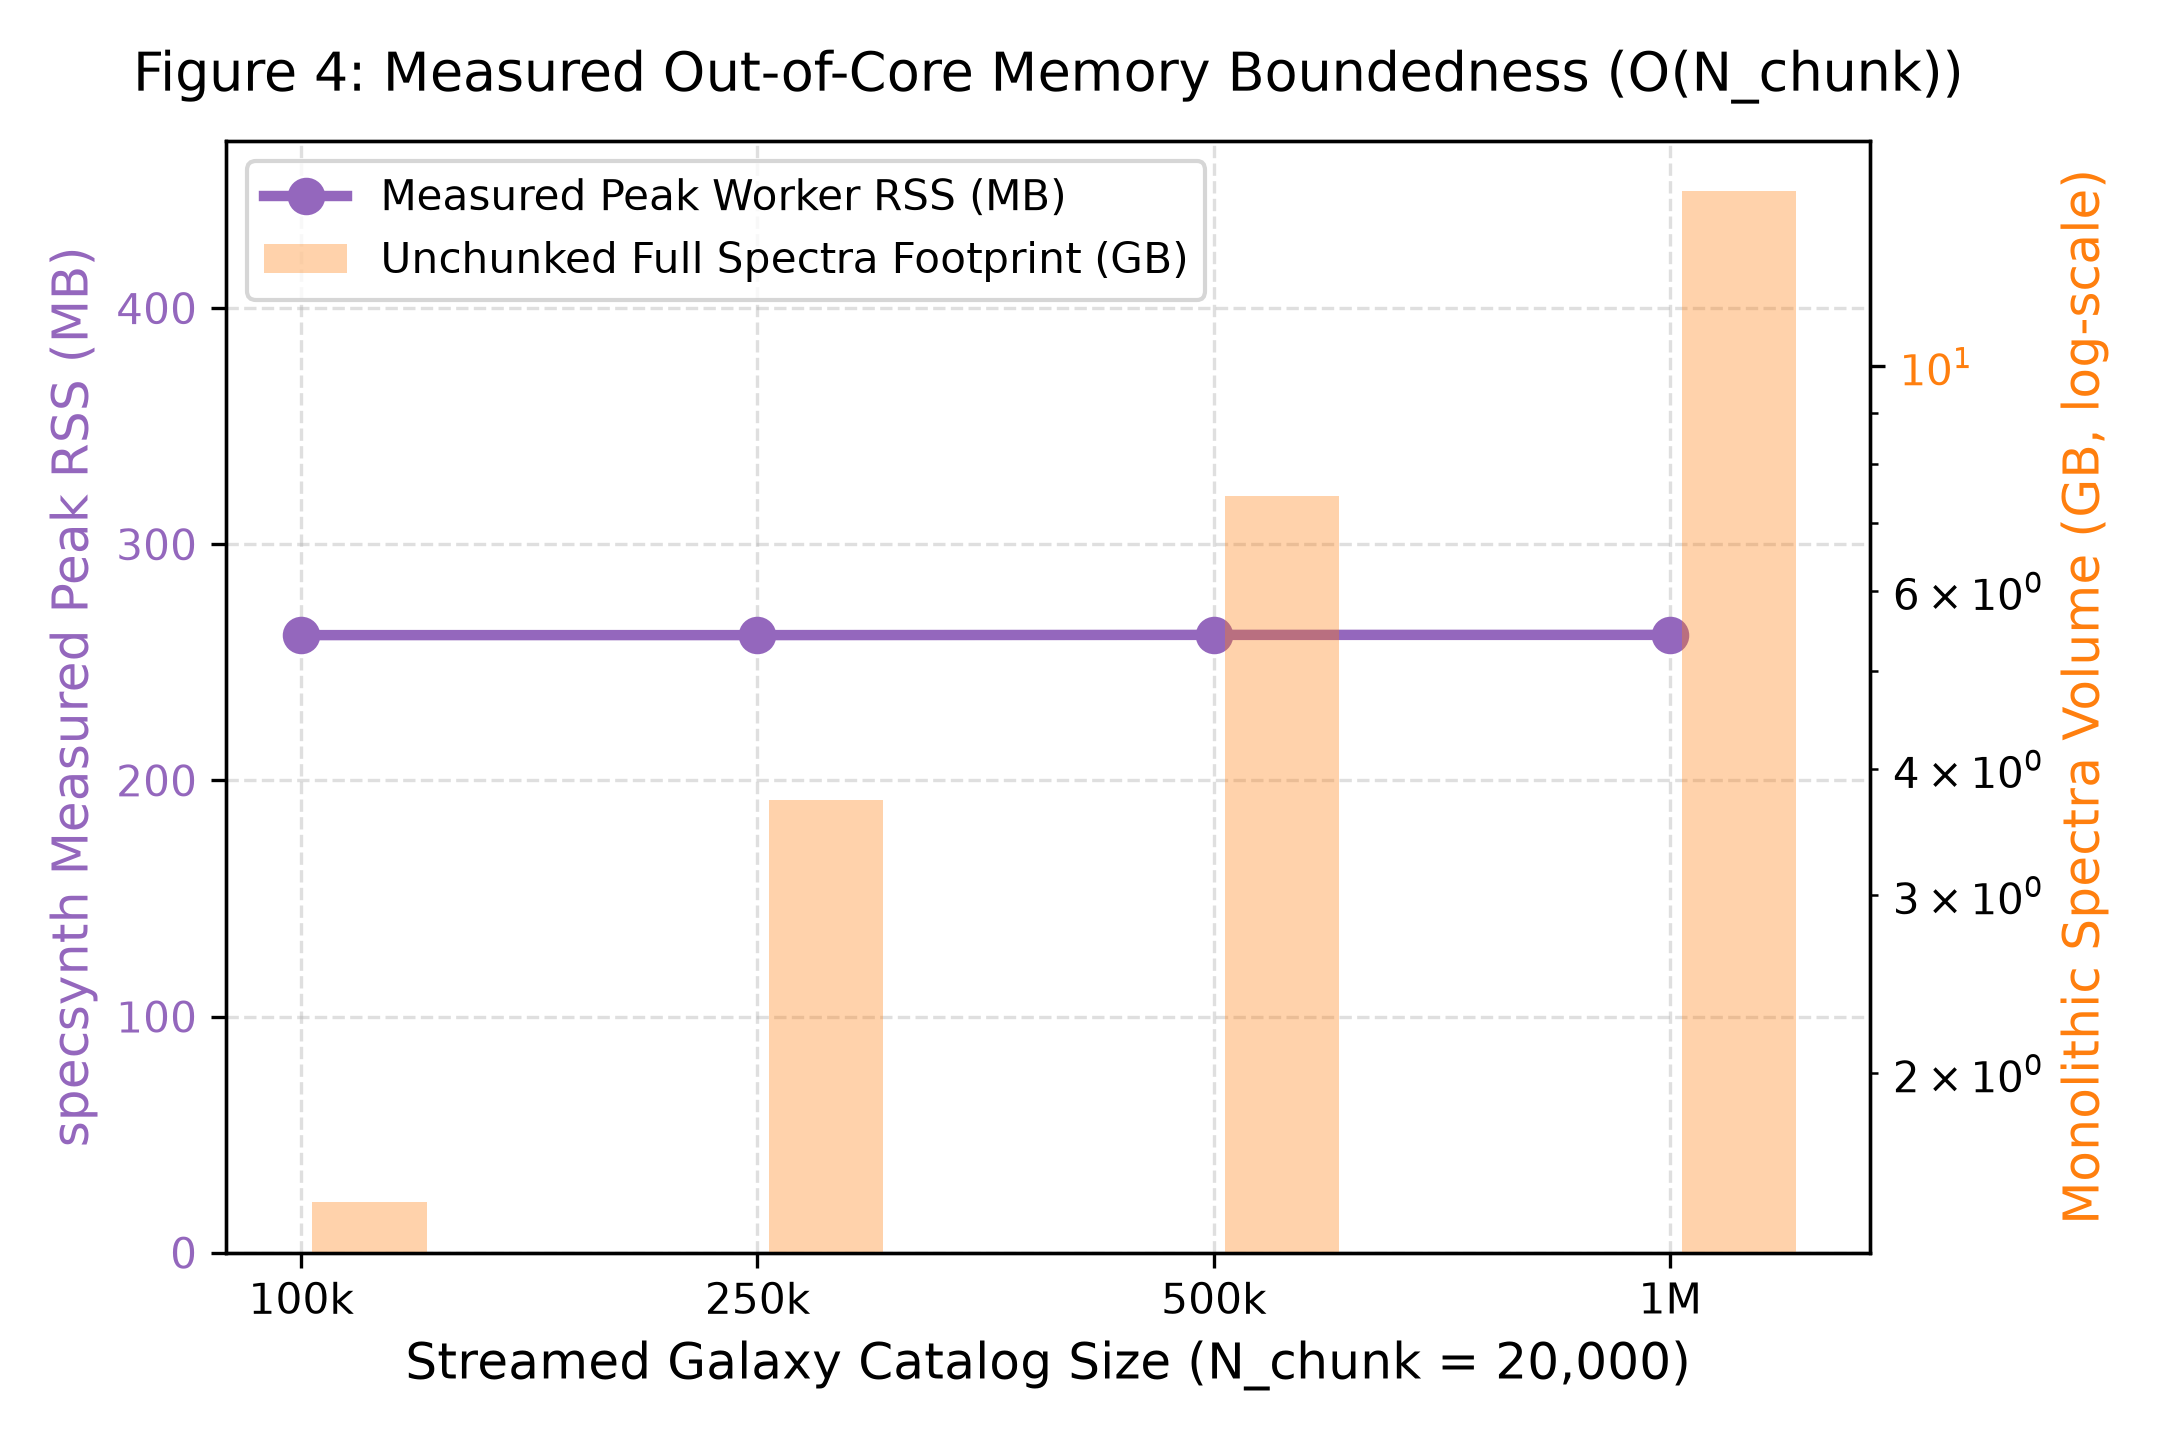
\includegraphics[width=0.78\textwidth]{figures/fig4_memory_usage.png}
\caption{Measured peak worker RSS (purple line, left axis) versus monolithic unchunked $W=4{,}000$ spectral memory volume (orange bars, right axis) across $10^5$ to $10^6$ streamed galaxies.}
\label{fig:memory}
\end{figure}

\subsection{Multi-Node Cloud Kubernetes vs.\ Local Multi-Worker Execution}
\label{sec:multinode}
To verify true multi-node distributed orchestration, we deployed \texttt{specsynth} on a 3-node Oracle Container Engine for Kubernetes (OKE) cluster using the Dask Kubernetes Operator (\texttt{VM.Standard.E3.Flex} AMD EPYC nodes; \texttt{paper/benchmark\_manifest\_oci\_oke\_3node.json}). Synthesizing $100{,}000$ galaxies ($K=120$, $W=2{,}000$, 5 chunks of 20,000, $z=2.0$, Madau IGM, 7 JWST NIRCam bands) completed in $1.86$~s ($53{,}814$~gal~s$^{-1}$, $51.7$~GFLOPS, estimated compute cost $\$0.000017$~USD) with a maximum relative error of $8.16\times 10^{-7}$ against the serial \texttt{float64} baseline.

For comparison, running multiple Dask worker processes on a single shared 12-core workstation (\texttt{paper/benchmark\_manifest\_cluster\_scaling.json}, $N=60{,}000$, $W=2{,}000$) scales from $13.24\pm 4.19$~s (1 worker, $4{,}531$~gal~s$^{-1}$) to $9.03\pm 0.30$~s (2 workers, $6{,}644$~gal~s$^{-1}$, $1.47\times$ speedup, $73\%$ efficiency), before degrading at 3 workers ($17.29\pm 1.36$~s) due to OpenBLAS thread oversubscription and memory-bus contention on one physical socket. This empirical contrast motivates \texttt{specsynth}'s dynamic CPU core budgeting and demonstrates why true multi-node horizontal scaling requires separate physical sockets or container CPU quotas.

\subsection{Analytical Multi-Node Scaling and Cloud Economics Projections}
\label{sec:analytical}
Because galaxy chunks are statistically independent and the read-only SSP matrix is persisted once peer-to-peer via \texttt{client.persist(ssp)}, scaling beyond 3 nodes is modeled analytically from the measured single-node baseline ($57{,}978$~gal~s$^{-1}$) under a conservative parallel-efficiency decay curve ($0.98$ at 2 workers down to $0.75$ at 64 workers; Figures~\ref{fig:strong_scaling} and~\ref{fig:weak_scaling}). For a fixed $10^7$-galaxy workload, analytical strong scaling projects $113{,}637$~gal~s$^{-1}$ ($88.0$~s) on 2 nodes, $431{,}357$~gal~s$^{-1}$ ($23.2$~s) on 8 nodes, $1{,}521{,}345$~gal~s$^{-1}$ ($6.6$~s) on 32 nodes, and $2{,}782{,}948$~gal~s$^{-1}$ ($3.6$~s) on 64 nodes. Analytical weak scaling at 500,000 galaxies per worker remains near-constant ($8.6$~s to $9.7$~s across 1--32 workers).

\begin{figure}[t]
\centering
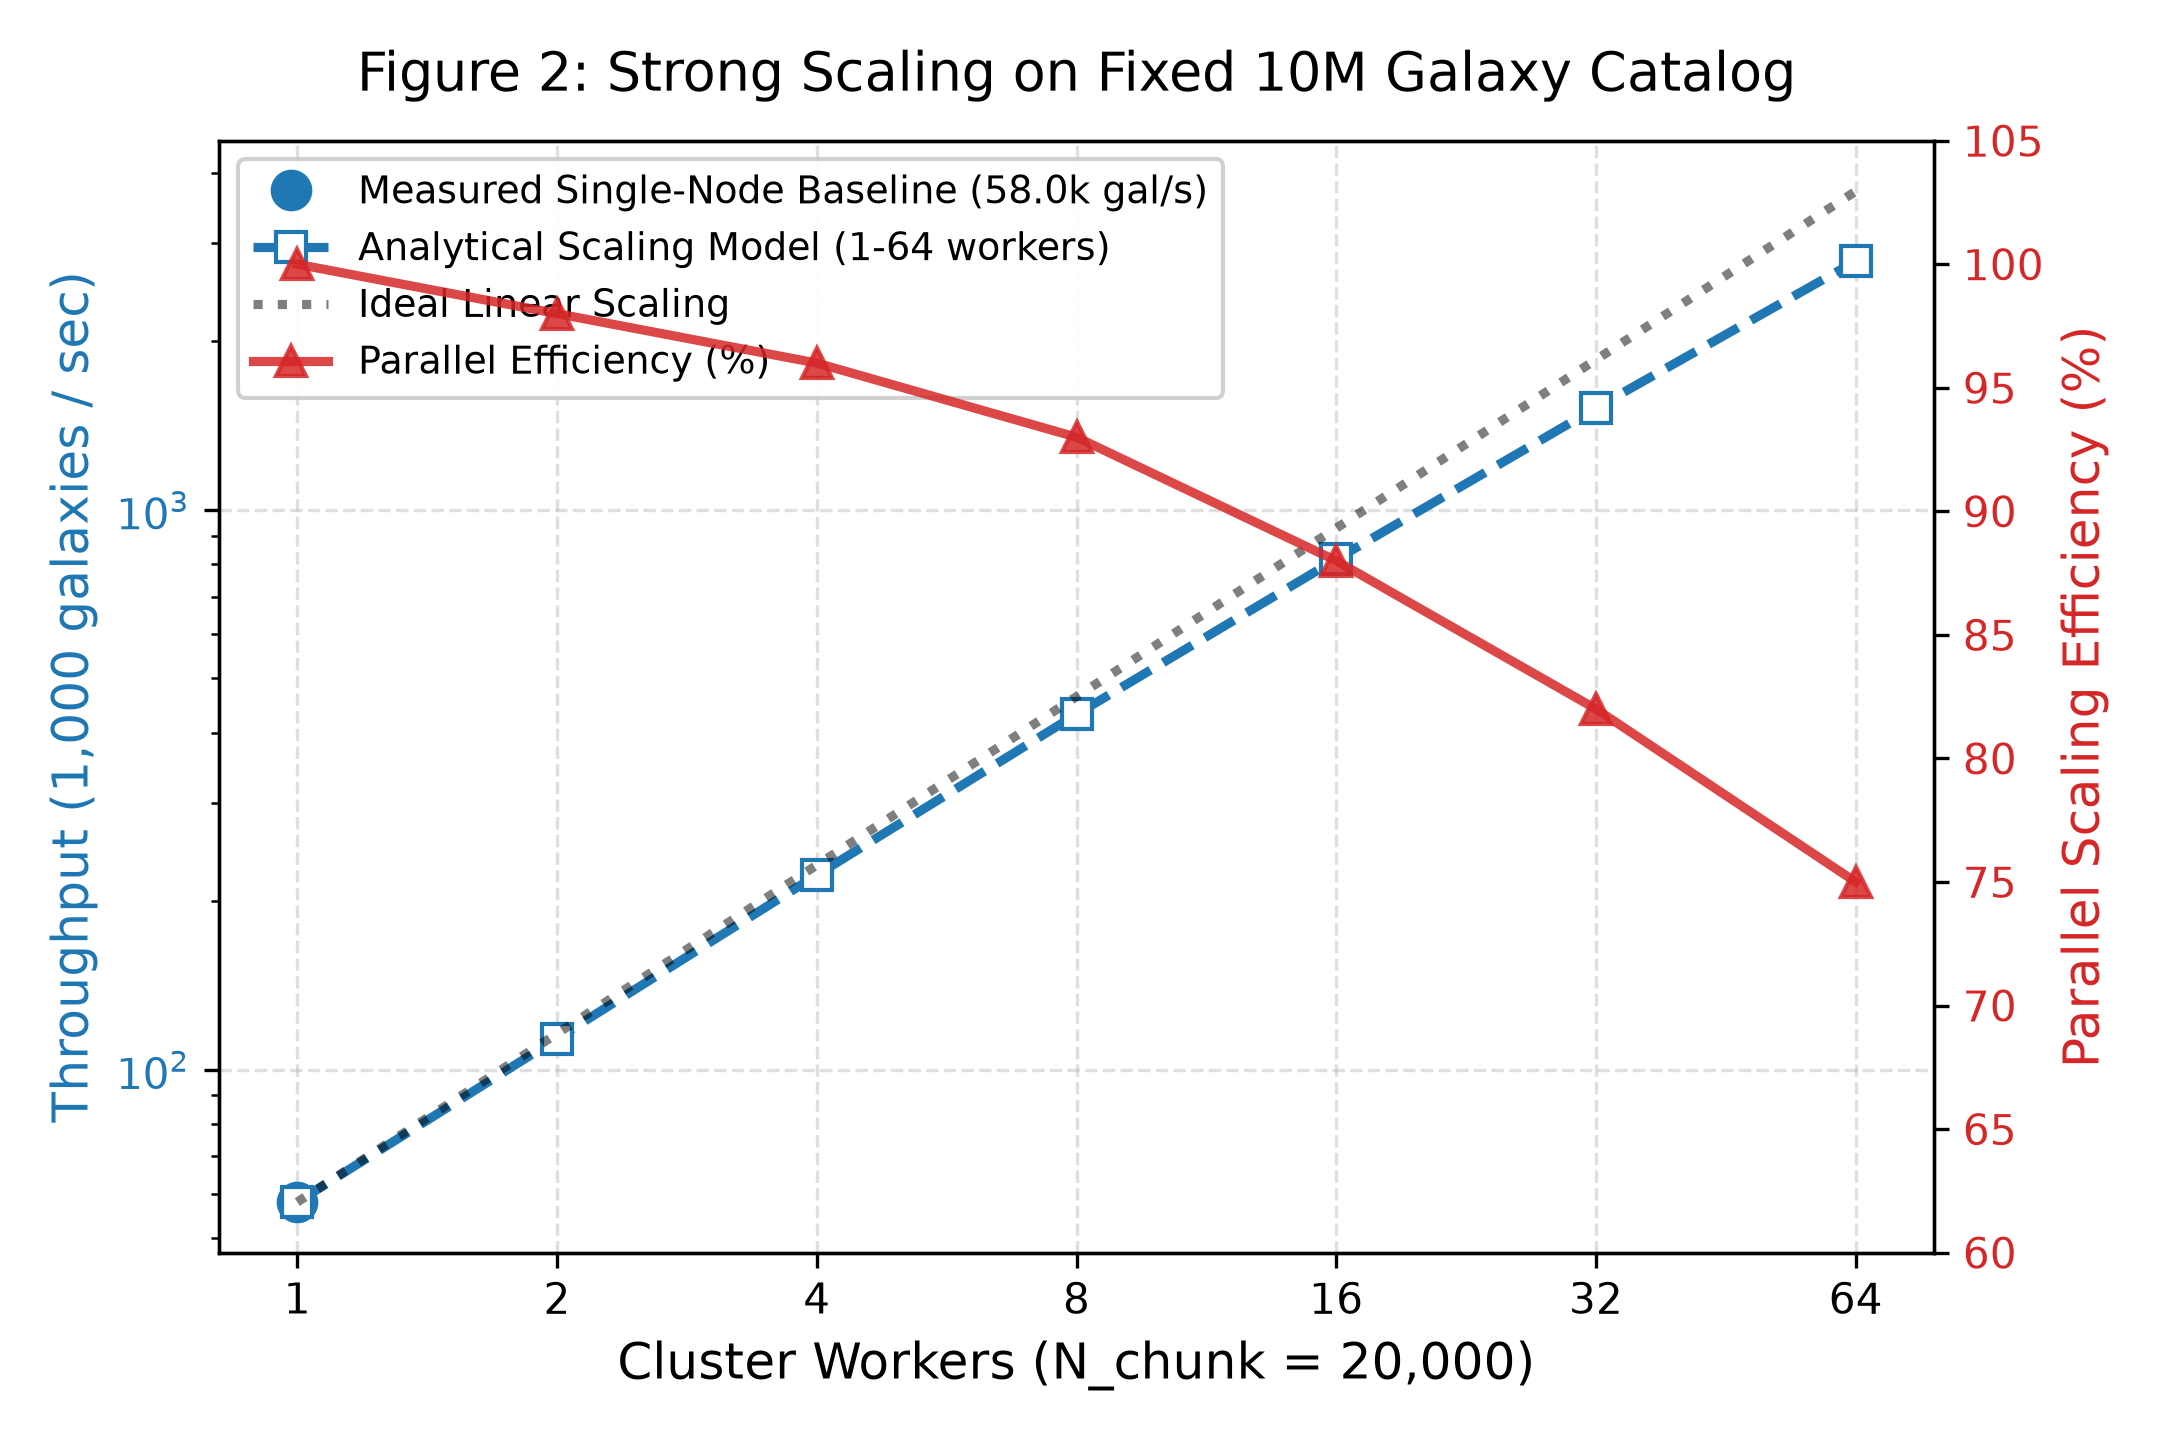
\includegraphics[width=0.78\textwidth]{figures/fig2_strong_scaling.png}
\caption{Analytical strong-scaling throughput and parallel efficiency on a fixed $10^7$-galaxy catalog anchored to the measured single-node CPU baseline ($57{,}978$~gal~s$^{-1}$).}
\label{fig:strong_scaling}
\end{figure}

\begin{figure}[t]
\centering
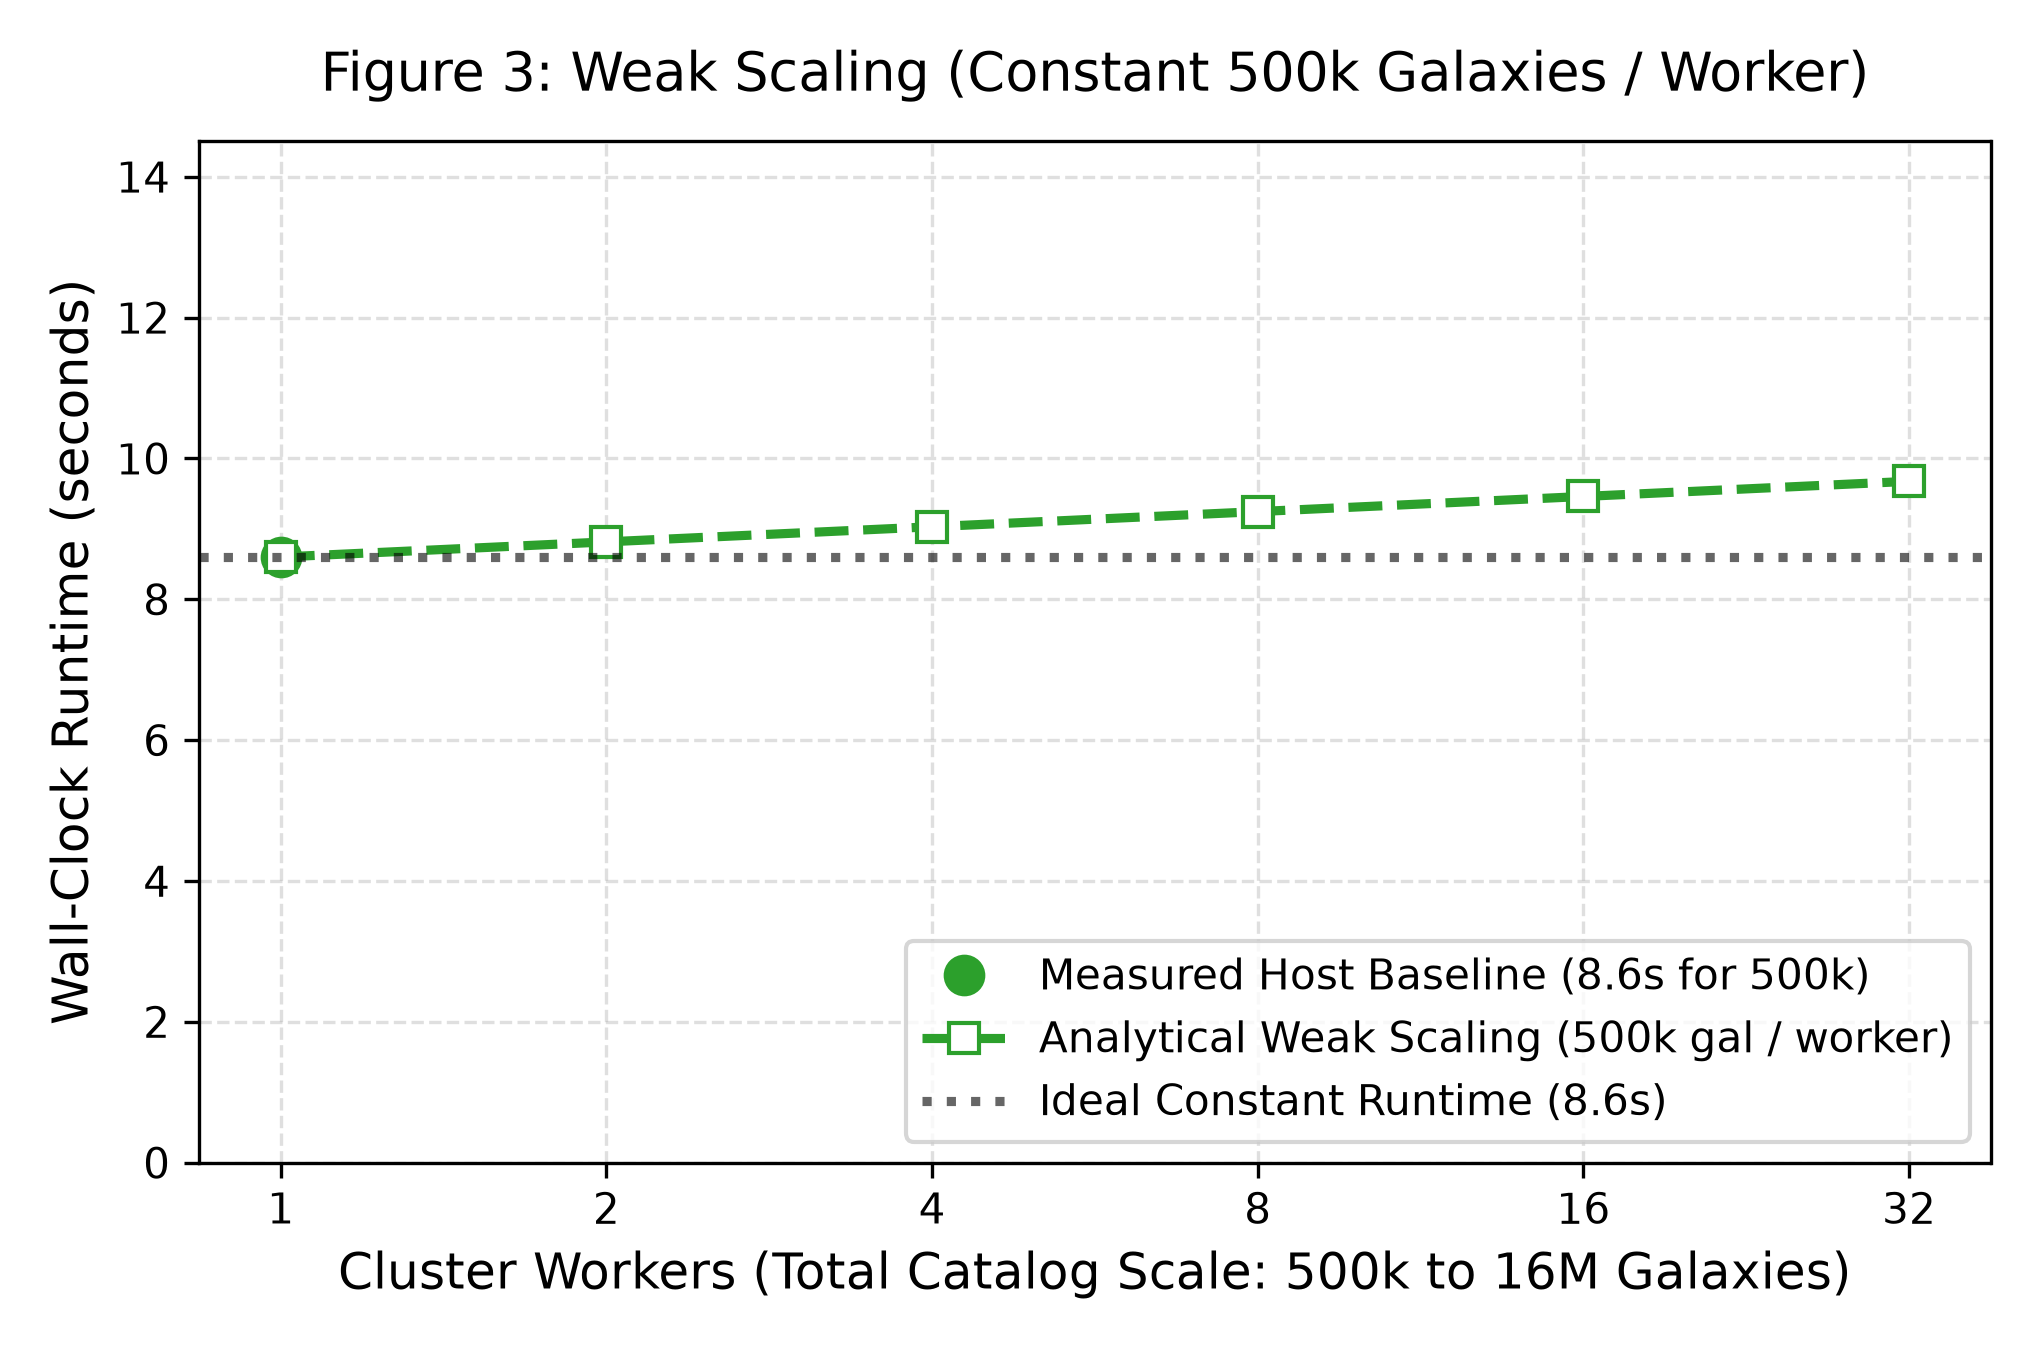
\includegraphics[width=0.78\textwidth]{figures/fig3_weak_scaling.png}
\caption{Analytical weak-scaling wall-clock runtime at a constant workload of $500{,}000$ galaxies per worker across 1--32 cluster nodes.}
\label{fig:weak_scaling}
\end{figure}

Combining this scaling model with representative cloud Spot VM pricing ($\$0.088\,\mathrm{hr}^{-1}$ per 8-vCPU node; Figure~\ref{fig:economics} and Table~\ref{tab:economics}) indicates that full 8-band photometric forward modeling of a $10^9$-galaxy survey catalog requires roughly $5.6$~minutes on 64 Spot nodes for $\sim \$4.20$~USD in compute while writing only $32$~GB of compressed photometry.

\begin{figure}[t]
\centering
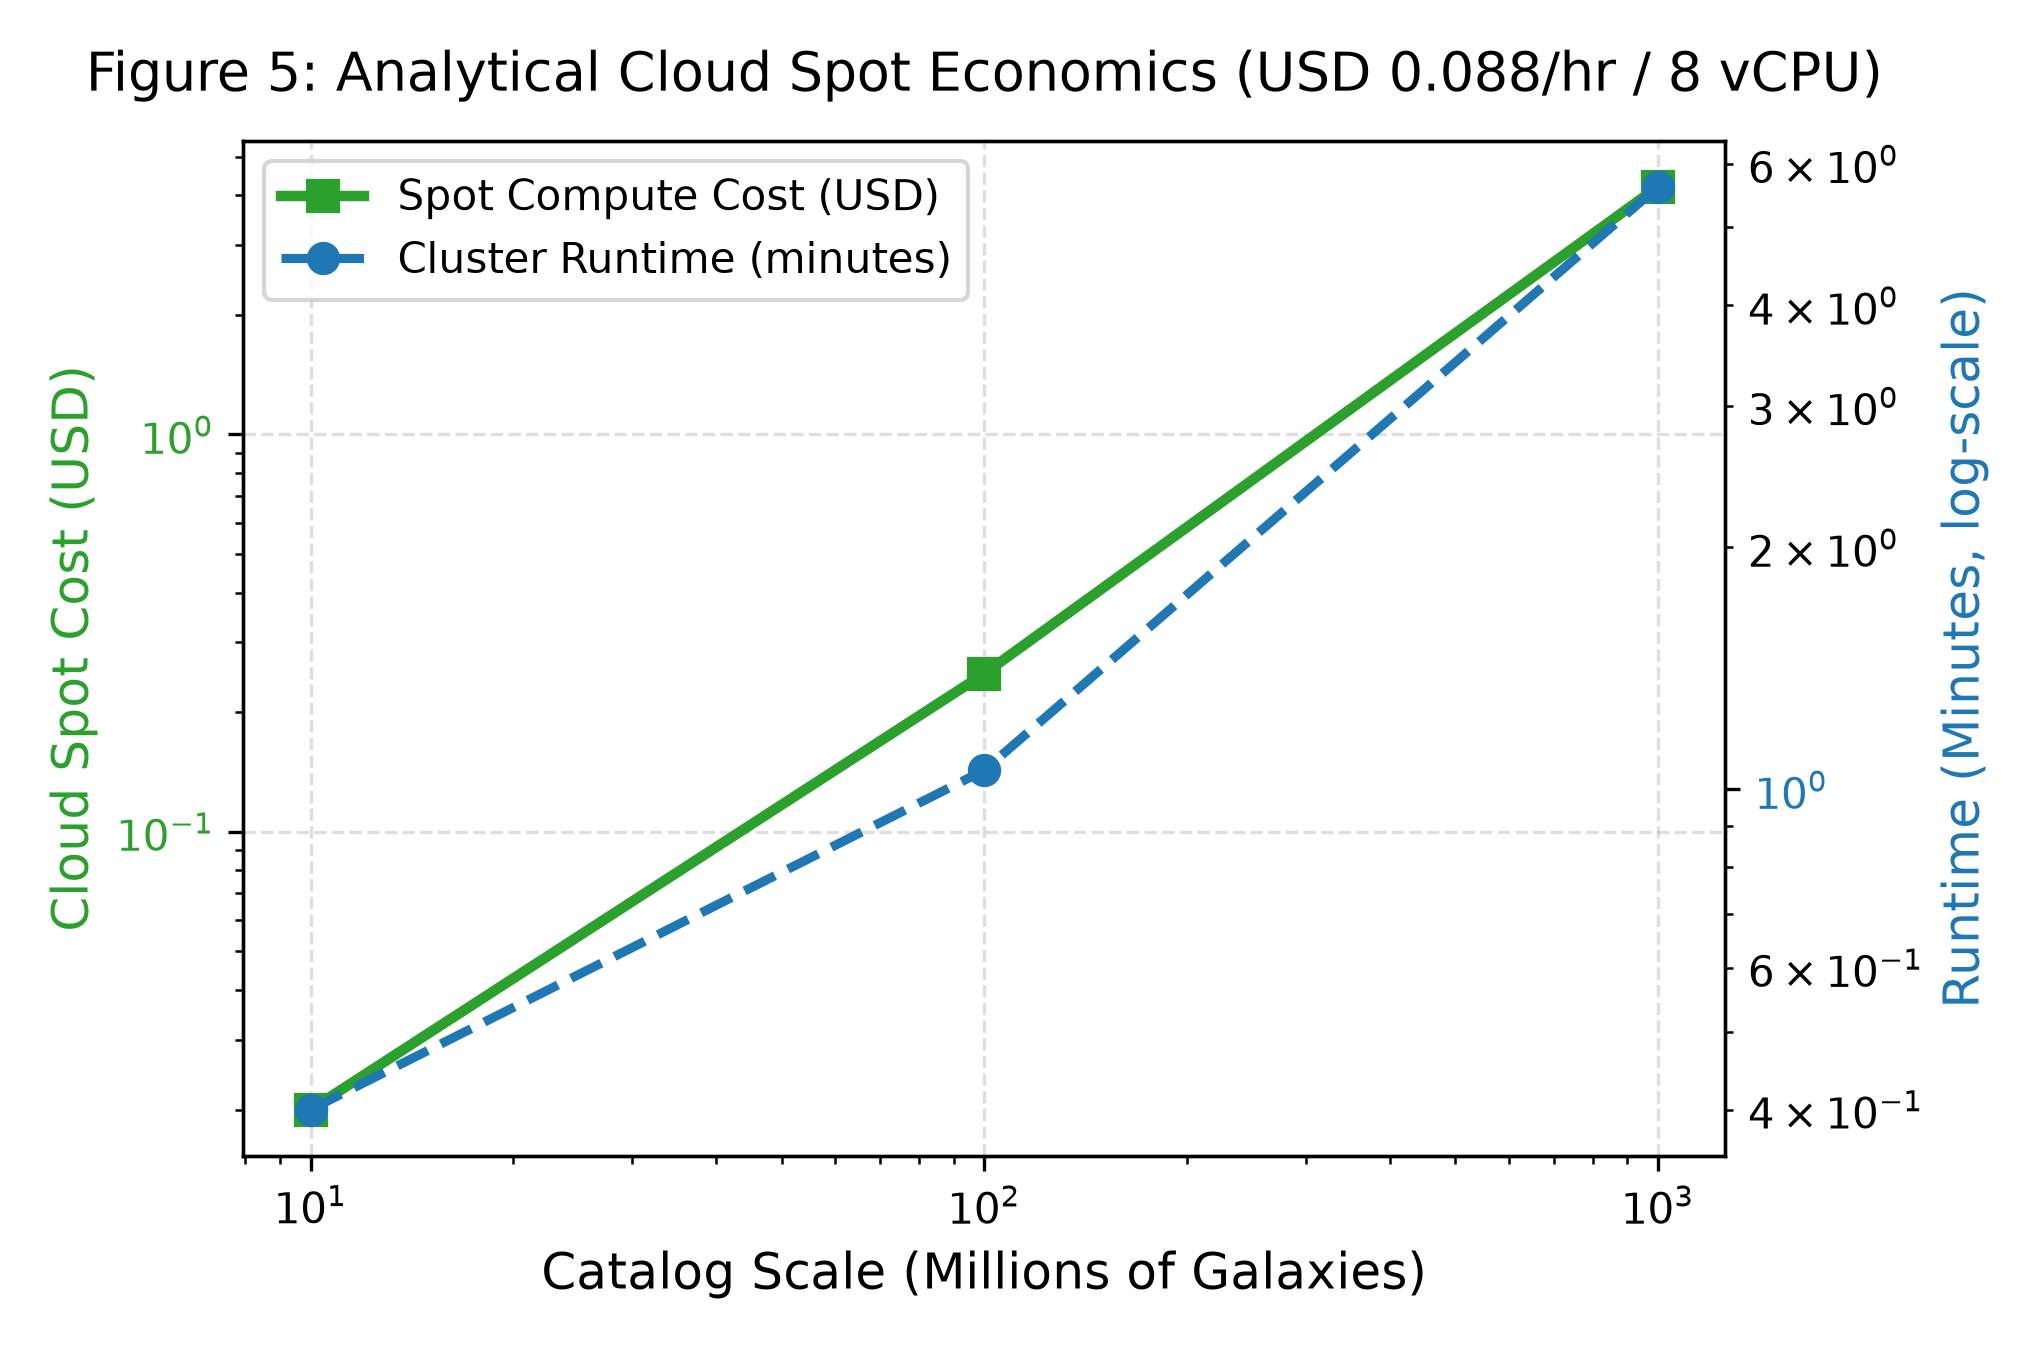
\includegraphics[width=0.76\textwidth]{figures/fig5_cloud_economics.png}
\caption{Analytical cloud Spot compute cost (green, left axis) and projected cluster runtime (blue, right axis) from $10^7$ to $10^9$ galaxies at $\$0.088\,\mathrm{hr}^{-1}$ per 8-vCPU Spot VM.}
\label{fig:economics}
\end{figure}

\begin{table}[t]
\centering
\caption{Analytical survey-scale photometry volume, runtime, and Spot compute cost projections (8 bands, $\$0.088\,\mathrm{hr}^{-1}$ per 8-vCPU VM).}
\label{tab:economics}
\small
\begin{tabular}{@{}rccc@{}}
\toprule
\textbf{Survey Catalog Scale} & \textbf{Photometry Output} & \textbf{Projected Runtime} & \textbf{Est.\ Spot Cost} \\
\midrule
10 Million Galaxies & 320~MB & $\sim 24$~s & $\sim \$0.02$~USD \\
100 Million Galaxies & 3.2~GB & $\sim 1.1$~min & $\sim \$0.25$~USD \\
1 Billion Galaxies & 32~GB & $\sim 5.6$~min (64 nodes) & $\sim \$4.20$~USD \\
\bottomrule
\end{tabular}
\end{table}

%% =========================================================================
\section{Scientific Demonstration: Synthetic JWST NIRCam Population}
\label{sec:science_demo}

To illustrate end-to-end astrophysical output beyond systems telemetry, we executed a 50,000-galaxy synthesis at $z=2.0$ with Charlot \& Fall two-component dust attenuation, Madau (1995) IGM transmission, and in-flight projection onto calibrated JWST NIRCam filters (\texttt{F090W}--\texttt{F444W}) via \texttt{scripts/generate\_paper\_figures.py}. The complete run---including parameter generation, SFH projection, cosmological redshifting, IGM transmission, and 7-band contraction---completed in $3.96$~s on a single CPU workstation (Figure~\ref{fig:jwst_demo}). Both the Color--Magnitude Diagram (\texttt{F200W}--\texttt{F444W} vs.\ \texttt{F200W}) and the high-$z$ two-color sequence (\texttt{F150W}--\texttt{F277W} vs.\ \texttt{F277W}--\texttt{F444W}) cleanly recover the expected dust-reddening vector and stellar-mass color locus.

\begin{figure*}[t]
\centering
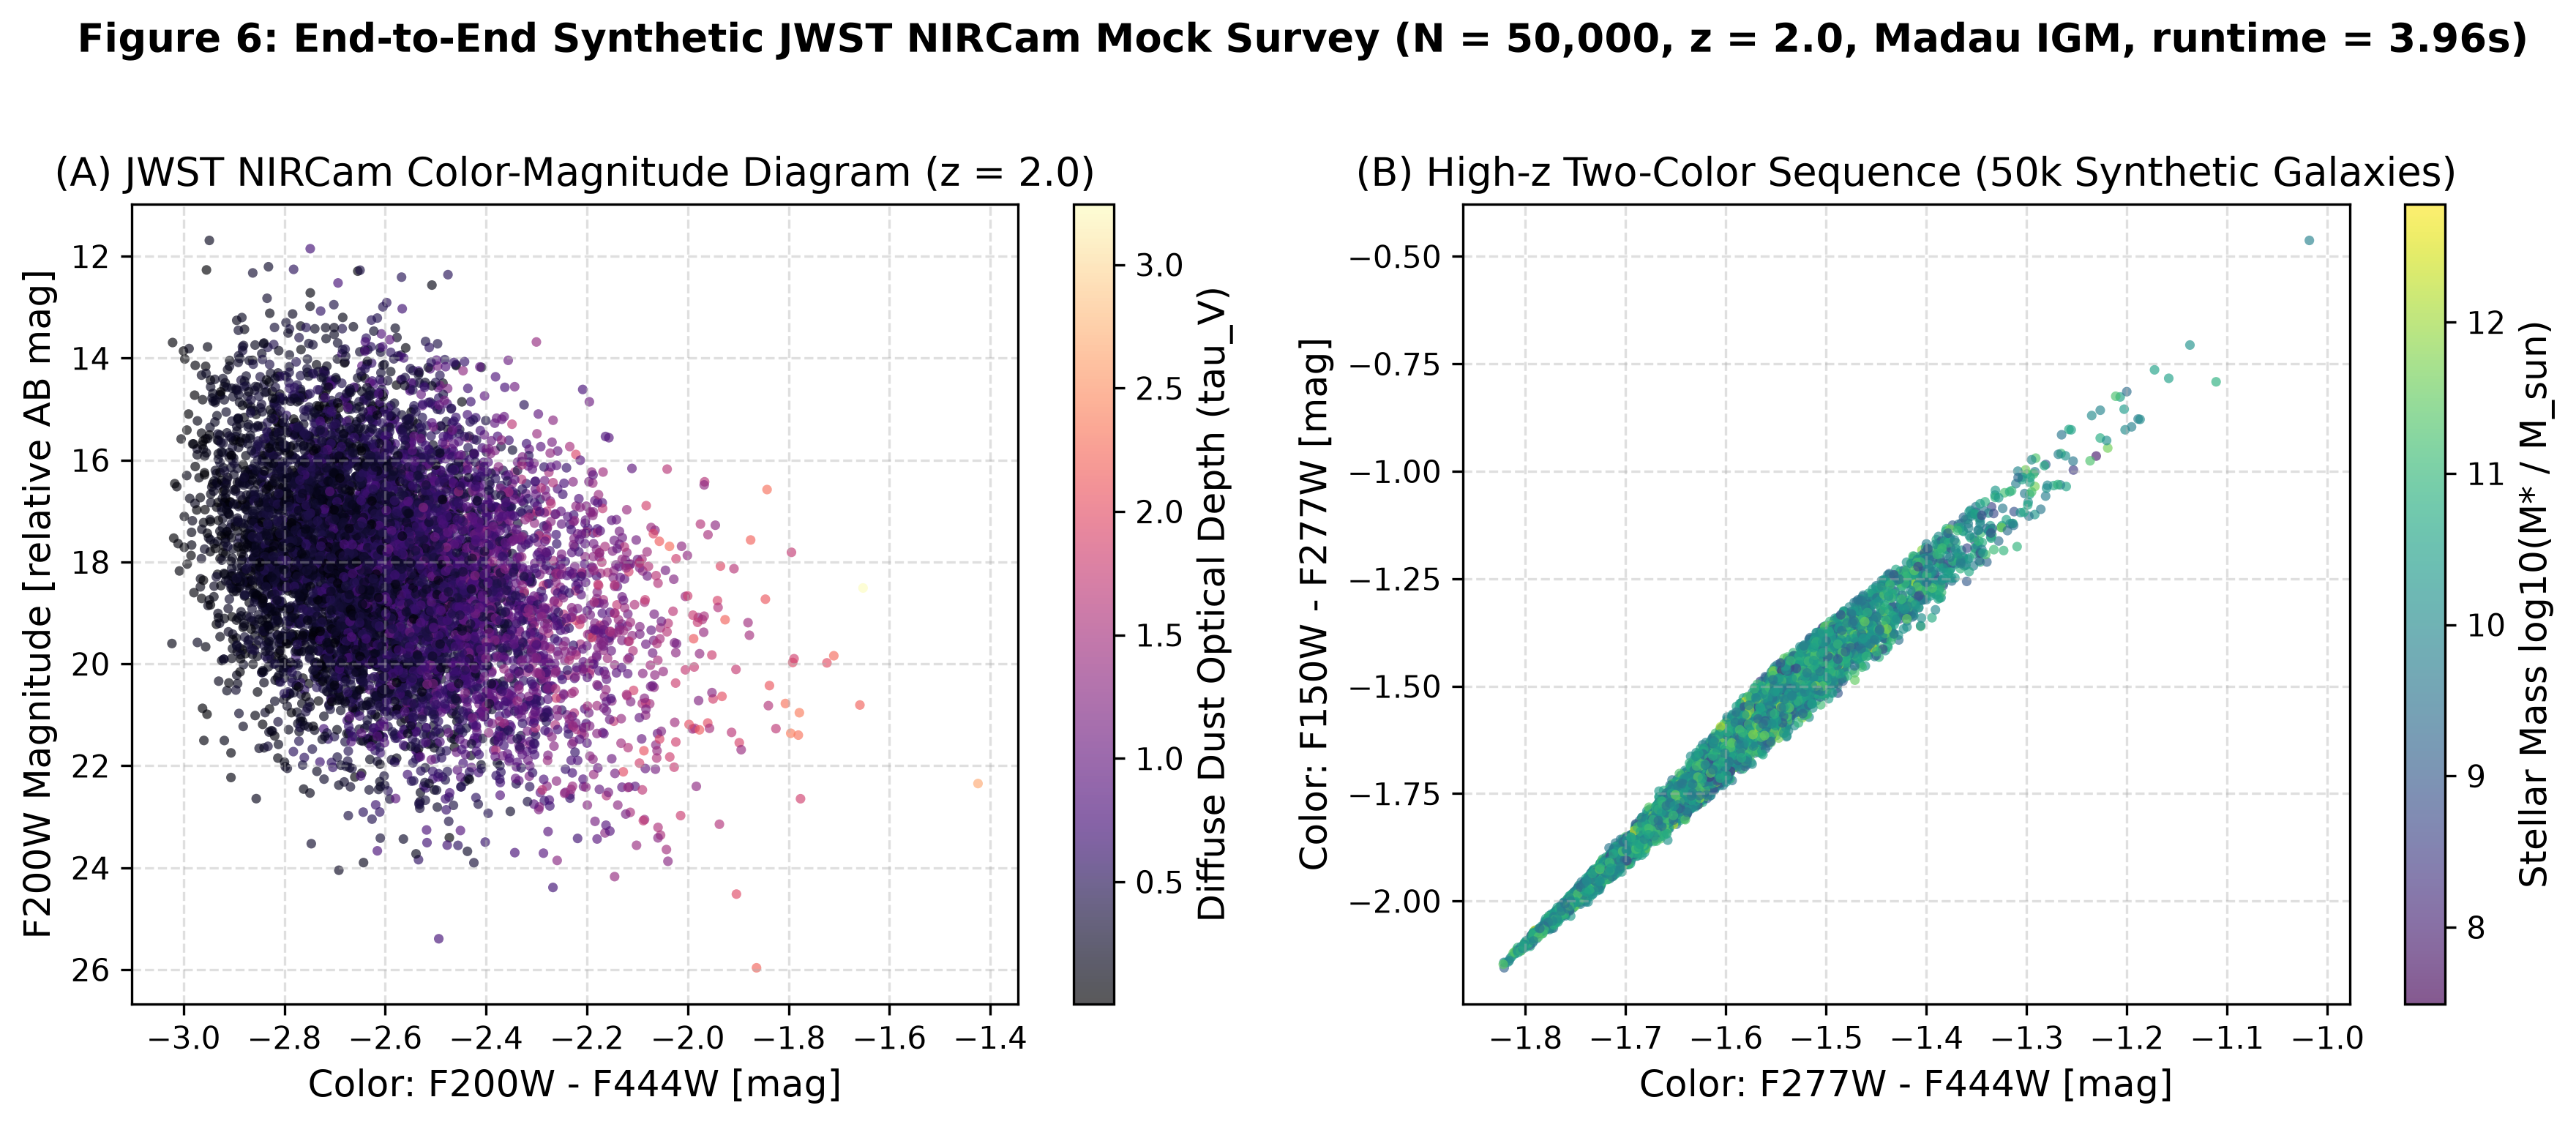
\includegraphics[width=\textwidth]{figures/fig6_jwst_science_demo.png}
\caption{End-to-end 50,000-galaxy synthetic JWST NIRCam mock survey at $z=2.0$ with Charlot \& Fall dust and Madau IGM attenuation (total runtime $3.96$~s on a single CPU host; 8,000 points plotted for visual clarity). (A)~Color--Magnitude Diagram colored by diffuse dust optical depth $\tau_V$. (B)~High-redshift two-color sequence colored by $\log_{10}(M_*/M_\odot)$.}
\label{fig:jwst_demo}
\end{figure*}

%% =========================================================================
\section{Limitations and Future Roadmap}
\label{sec:limitations}

Several boundaries define the current scope of \texttt{specsynth} v1.0.0:
\begin{itemize}
\item \textbf{Empirical vs.\ Projected Cluster Scale:} Multi-node Kubernetes execution has been empirically measured up to 3 physical cloud VM nodes ($53{,}814$~gal~s$^{-1}$ on OCI OKE), whereas 16--64 node estimates in Section~\ref{sec:analytical} remain analytical extrapolations subject to real-world object-store rate limits and scheduler latency.
\item \textbf{Physical Scope:} \texttt{specsynth} targets population-scale continuum synthesis, two-component dust, cosmological dimming, Madau IGM transmission, and broadband photometry. It intentionally omits nebular radiative-transfer photoionization, line-of-sight velocity dispersion broadening, and active galactic nucleus (AGN) emission, which are better handled by specialized codes such as \texttt{Synthesizer} \citep{lovell2025synthesizer} or \texttt{Prospector} \citep{johnson2021prospector} and can be incorporated in future adapter extensions via pre-computed nebular+stellar SSP grids.
\item \textbf{Live External Code Hooks:} Automated CI validates cosmology and \texttt{float64} photometry on every commit, while live \texttt{python-fsps} and \texttt{DSPS} cross-comparisons remain optional extras due to external Fortran/JAX build dependencies.
\end{itemize}

%% =========================================================================
\section{Conclusion}
\label{sec:conclusion}

\texttt{specsynth} demonstrates that reformulating composite stellar population synthesis as an out-of-core, mixed-precision Zarr/Dask/CuPy streaming pipeline eliminates multi-terabyte intermediate spectral storage while preserving sub-micromag ($<3\times 10^{-7}$~mag) photometric fidelity against independent \texttt{float64} baselines. With bounded worker RAM ($261.5$--$261.8$~MB across a $10\times$ catalog expansion), $4.51\times$ GPU acceleration on commodity cloud hardware, verified 3-node Kubernetes scaling, an automated four-tier scientific quality sentry, and an archived 100,000-galaxy reference benchmark catalog, \texttt{specsynth} provides a reproducible, cloud-native foundation for next-generation mock survey pipelines.

%% =========================================================================
\section*{CRediT Authorship Contribution Statement}
\textbf{Sankar Ganesh:} Conceptualization, Methodology, Software, Validation, Formal analysis, Investigation, Data curation, Writing -- original draft, Writing -- review \& editing, Visualization.

\section*{Declaration of Generative AI and AI-Assisted Technologies in the Writing Process}
During the development of \texttt{specsynth} and preparation of this work, the author used generative AI coding and writing assistants (Google Gemini / Antigravity and Claude-class models) to assist with unit-test scaffolding, documentation drafting, CLI/adapter boilerplate refactoring, and manuscript language editing. After using these tools, the author reviewed, verified, and edited all scientific framing, astrophysical equations, software architecture, numerical validation tolerances, benchmark executions, and manuscript text, and takes full responsibility for the content of the publication.

\section*{Declaration of Competing Interest}
The author declares that he has no known competing financial interests or personal relationships that could have appeared to influence the work reported in this paper.

\section*{Data and Code Availability}
\texttt{specsynth} v1.0.0 is released openly under the MIT License at \url{https://github.com/SankarGaneshb/specsynth}, with online documentation at \url{https://sankarganeshb.github.io/specsynth/} and container images published at \texttt{docker.io/bsankarganesh/specsynth}. (An archival Zenodo software release DOI will be minted from the tagged v1.0.0 release prior to final publication.) The canonical 100,000-galaxy lightcone reference benchmark catalog (\texttt{specsynth-benchmark-100k}, $z\in[0.05, 3.8]$, 16 calibrated JWST/HST/SDSS bands in \texttt{float64}, Parquet and Zarr formats) is permanently archived on Hugging Face under DOI \href{https://doi.org/10.57967/hf/11635}{\texttt{10.57967/hf/11635}} \citep{sankar_ganesh_bala_krishnan_2026}.

\section*{Acknowledgements}
The author gratefully acknowledges the foundational theoretical and software contributions enabling this work: St\'ephane Charlot and S.~Michael Fall for the two-component dust attenuation formulation \citep{charlot2000simple}; Piero Madau for the analytic IGM transmission model \citep{madau1995radiative}; the authors of public SSP libraries (BC03, FSPS, E-MILES, BPASS); and the open-source communities maintaining Dask, Zarr, NumPy, CuPy, and Astropy.

%% =========================================================================
\appendix
\section{Benchmark Provenance and Reproducibility Manifests}
\label{app:provenance}

All empirical measurements reported in Section~\ref{sec:benchmarks} are archived in machine-readable JSON manifests inside the \texttt{paper/} directory of the repository:

\begin{itemize}
\item \textbf{Host 1 -- Local Verification Workstation} (\texttt{paper/benchmark\_manifest.json}): Windows~11 (\texttt{10.0.26300}), Intel 12 physical cores / 14 logical threads, 15.49~GB RAM, \texttt{scipy-openblas}, Python~3.13.1, NumPy~2.5.4, Dask~2026.8.0, Zarr~3.4.2, Astropy~8.0.2, commit \texttt{a718e9e4}, timestamp \texttt{2026-11-11T16:06:09Z}.
\item \textbf{Host 2 -- Cloud NVIDIA Tesla T4 GPU Node} (\texttt{paper/benchmark\_manifest\_gpu\_t4.json}): Linux~6.18.55+ x86\_64 (2C/4T, 31.35~GB RAM), NVIDIA Tesla T4 (14.56~GB VRAM, CUDA~12.2, CuPy~13.3.0), Python~3.13.16, NumPy~2.1.2, Dask~2024.12.0, Zarr~2.18.2, timestamp \texttt{2026-11-13T15:19:21Z}.
\item \textbf{Host 3 -- 3-Node Cloud Kubernetes Cluster} (\texttt{paper/benchmark\_manifest\_oci\_oke\_3node.json}): Oracle Cloud Infrastructure OKE, 3 dedicated \texttt{VM.Standard.E3.Flex} nodes (Oracle Linux~8.10, CRI-O~1.36.3, \texttt{dask-kubernetes-operator} 2026.3.0), container digest \texttt{sha256:fb6d2bbd...}, timestamp \texttt{2026-11-15T01:26:51+05:30}.
\item \textbf{Host 4 -- Local Multi-Worker Contention Manifest} (\texttt{paper/benchmark\_manifest\_cluster\_scaling.json}): 1-, 2-, and 3-worker local comparison ($N=60{,}000$, $N_{\text{chunk}}=20{,}000$, $W=2{,}000$), commit \texttt{7cb84e46}, timestamp \texttt{2026-11-15T18:22:24Z}.
\item \textbf{Cross-Validation Manifest} (\texttt{paper/cross\_validation\_manifest.json}): Planck~2018 / concordance cosmology verification and 500-galaxy 16-band IllustrisTNG-like photometric verification against independent \texttt{float64} baselines, timestamp \texttt{2026-11-18T13:55:21Z}.
\end{itemize}

\noindent Key reproduction commands from the repository root:
\begin{lstlisting}[language=bash]
# Automated unit & integration test suite (159 tests)
pytest -v --cov=specsynth

# Cross-code cosmology & 16-band photometric validation
python scripts/cross_validate_sps.py --n-gal 500

# Scientific Sentry audit & autonomous remediation
python specsynth.py sentry --base ./run --sample 50000 --output ./run/sentry_report.json
python specsynth.py sentry-agent --base ./run --auto-remediate

# Hardware CPU/GPU benchmark & figure regeneration
python specsynth.py benchmark --n-gal 50000 --n-runs 5 --gpu \
       --output paper/benchmark_manifest_gpu_t4.json
python scripts/generate_paper_figures.py
\end{lstlisting}

\bibliographystyle{elsarticle-harv}
\bibliography{references}

\end{document}
